A continuación, se describen los resultados obtenidos del proceso de detección de temas tendencia con base en el procedimiento previamente descrito para cada uno de los idiomas seleccionados.

\subsection{Inglés}
\subsection{Español}

El proceso de \textit{clustering} hecho con base en el método K-means para el idioma español arrojó los resultados que se pueden ver en la figura \ref{fig:es_kmeans}. Se decidió probar diferente número de grupos con el fin de analizar el comportamiento y la exactitud con la que el algoritmos K-means es capaz de separarlos. Inicialmente, se probó con un total de cinco (\textit{véase fig} \ref{fig:es_kmeans_5}) \textit{clusters}, evidenciando que la separación entre los grupos color azul y morado era regular además del serio agravante de que a simple vista no es posible identificar el quinto \textit{cluster}. Se decidió entonces probar con un menor número grupos, o6bteniendo los resultados visibles en la figura \ref{fig:es_kmeans_4}, la cual resulta muy similar al caso previamente descrito.\\

Posteriormente, se redujo nuevamente el número de grupos definiéndolo en tres (\textit{véase fig} \ref{fig:es_kmeans_3}). En este caso las barreras de separación de cada grupo son completamente claras y son realmente pocos los documentos que las sobrepasan. Sin embargo, con base en el comportamiento a lo largo del tiempo se decidió intentar reducir el número de grupos a 2, obteniendo los resultados mostrados en la figura \ref{fig:es_kmeans_2}, en donde la división de \textit{clusters} es visible, pero la gráfica de comportamiento en el tiempo muestra mejores resultados.

\begin{figure}
     \centering
     \begin{subfigure}[b]{0.4\textwidth}
         \centering
         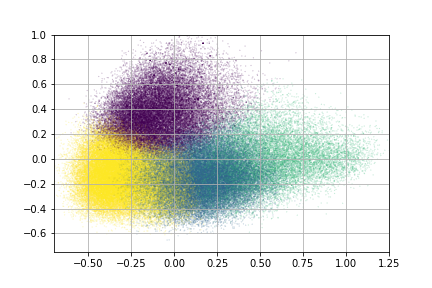
\includegraphics[width=\textwidth]{results/TopicDetection/es/PCA_2.png}
         \caption{2 clusters}
         \label{fig:es_kmeans_2}
     \end{subfigure}
     \hfill
     \begin{subfigure}[b]{0.4\textwidth}
         \centering
         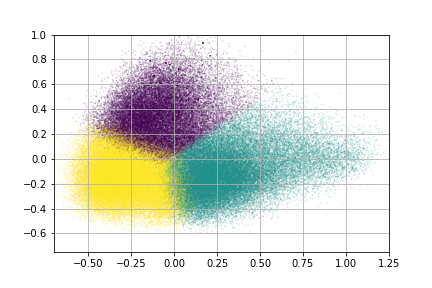
\includegraphics[width=\textwidth]{results/TopicDetection/es/PCA_3.png}
         \caption{3 clusters}
         \label{fig:es_kmeans_3}
     \end{subfigure}
     \hfill
     \begin{subfigure}[b]{0.4\textwidth}
         \centering
         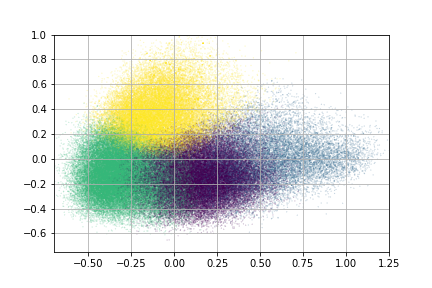
\includegraphics[width=\textwidth]{results/TopicDetection/es/PCA_4.png}
         \caption{4 clusters}
         \label{fig:es_kmeans_4}
     \end{subfigure}
     \hfill
     \begin{subfigure}[b]{0.4\textwidth}
         \centering
         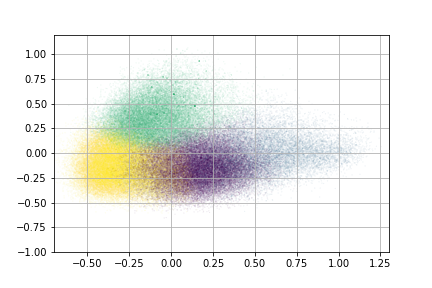
\includegraphics[width=\textwidth]{results/TopicDetection/es/PCA_5.png}
         \caption{5 clusters}
         \label{fig:es_kmeans_5}
     \end{subfigure}
        \caption{Resultados de K-means con diferente número de clusters}
        \label{fig:es_kmeans}
\end{figure}

Una vez seleccionado el número óptimo de grupos, se procede a extraer las palabras más representativas de cada uno de los grupos, mediante una nube de palabras. Se decide eliminar algunas que aparecen en mayoría en todos los \textit{clusters} con el fin de poder visualizar más aquellas que caracterizan cada uno.

\begin{figure}
     \centering
     \begin{subfigure}[b]{0.75\textwidth}
         \centering
         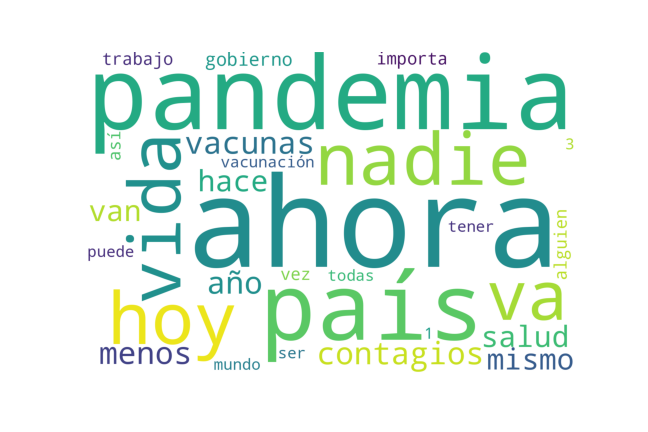
\includegraphics[width=\textwidth]{results/TopicDetection/es/cluster0.png}
         \caption{Cluster 0}
         \label{fig:es_c0}
     \end{subfigure}
     \hfill
     \begin{subfigure}[b]{0.75\textwidth}
         \centering
         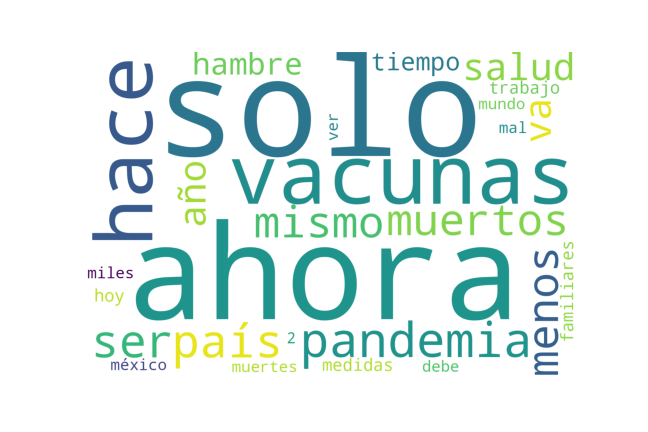
\includegraphics[width=\textwidth]{results/TopicDetection/es/cluster1.png}
         \caption{Cluster 1}
         \label{fig:es_c1}
     \end{subfigure}
        \caption{Principales palabras de cada uno de los clusters}
        \label{fig:es_clusters}
\end{figure}

Con base en las figuras \ref{fig:es_clusters} y \ref{fig:es_time} Es completamente evidente que el \textit{cluster} 1 crece fuertemente hacia el final de los meses evaluados, debido a la palabra vacunación, la cual ha sido tendencia últimamente y no aparece en el \textit{cluster} 0, cuya participación se reduce al final de los meses. De manera similar, los clusters presentan una tendencia opuesta en el inicio de los meses, debido quizás a la palabra nuevos, que esta presente únicamente en el \textit{cluster} 1.

\begin{figure}
    \centering
    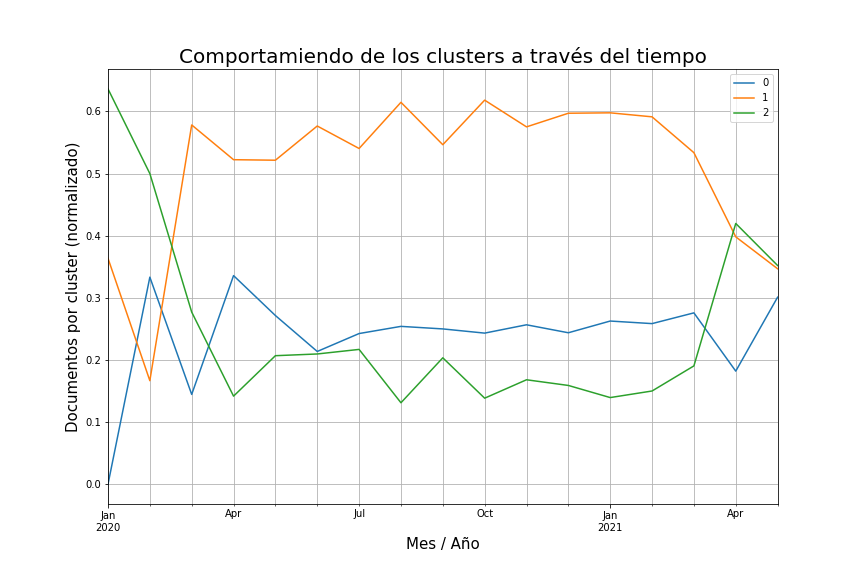
\includegraphics[width=0.9\textwidth]{results/TopicDetection/es/cluster_over_time.png}
    \caption{Comportamiento de los clusters en el tiempo}
    \label{fig:es_time}
\end{figure}

\subsection{Francés}